\documentclass{article}
\usepackage{graphicx}
\usepackage{gensymb}
\usepackage{graphicx}
\usepackage[left=2cm, top=3cm, a4paper, text={17cm, 24cm}]{geometry}

\usepackage{amsmath}
\usepackage{amsfonts}
\usepackage{amsthm}

\title{Project Blueberry}
\author{xhajekj00 }
\date{May 2026}

\begin{document}
\begin{titlepage}
    \begin{center}
        \Huge
        \textsc{ Vysoké učení technické v~Brně}\\
        \LARGE
        \textsc{ Fakulta elektrotechniky a komunikačních technologií}\\

        \vspace{\stretch{0.382}}
        \Large
        BPC-PRP\\
        \Huge
        Project Blueberry
        \vspace{\stretch{0.618}}

    \end{center}

    {\Large \today \hfill
    \begin{tabular}{@{}l l r@{}}
        Jan Hájek & (wekknsie)\\
        Volodymyr-Mykhailo Horbal & (MrVova)
    \end{tabular}
    }
\end{titlepage}

\section{Úvod}
Základ projektu tvoří univerzální robotizovaný systém Fenrir. Fenrir představuje již hotového robota, který zahrnuje všechny potřebné senzory a je založen na ROS2. Cílem projektu Blueberry bylo naprogramovat tohoto robota s využitím jeho možností tak, aby mohl samostatně opustit labyrint v rámci předmětu BPC-PRP. Za tímto účelem byly vytvořeny nody, které jsou součástí implementace ROS2, v nichž bylo soustředěno řešení.

\section{Architektura}
Celý systém je implementován pomocí samostatných ROS2 nodů, které zajišťují správný chod robota.

\begin{figure}[ht]
   \centering
   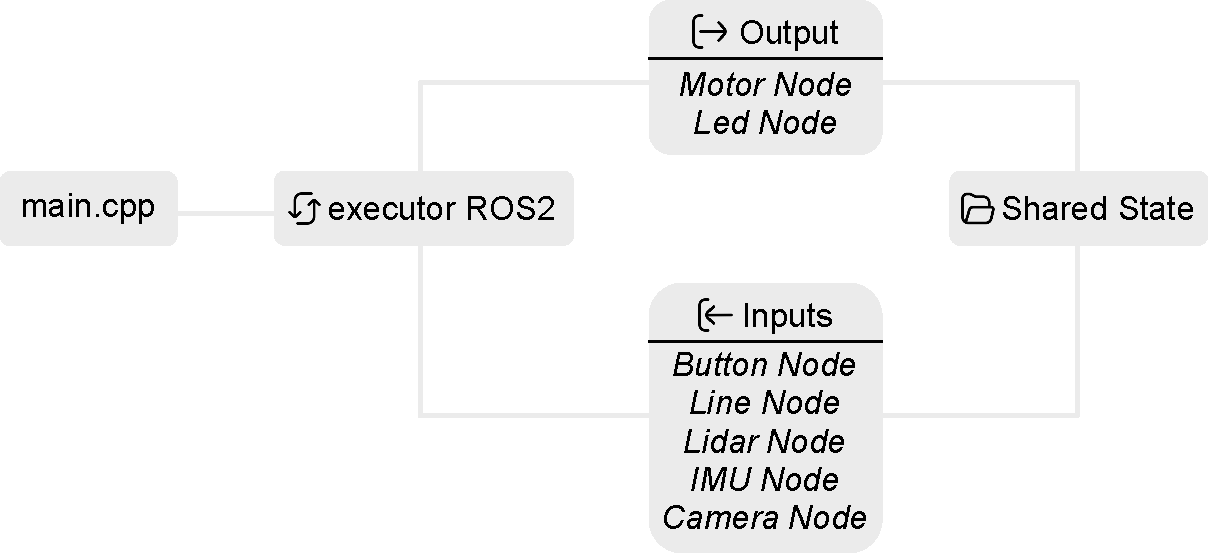
\includegraphics[width=0.6\linewidth]{figs/diagram.pdf}
   \caption{Grafické zobrazení jednotlivých částí}
\end{figure}

\subsection{Tlačítka}
Na vrchní části má robot umístěná tři tlačítka, kterými se spouští a ukončuje běh programu.

\subsection{LED}
Čtyři RGB diody, jenž leží vedle tlačítek, mají za úkol předávat informace jako je, čím se zrovna robot řídí, nebo která stěna je příliš blízko. Značí taktéž úspěšnou kalibraci IMU senzoru. 

\subsection{IMU senzor}
Abychom dokázali s přesností zatáčet a držet robota uprostřed koridoru využíváme senzor IMU abychom měli údaje o jeho natočení a směru. K zajištění správnosti dat je nutno senzor při zapnutí programu kalibrovat a to sběrem dat při nehybnosti. 

\begin{figure}[ht]
   \centering
   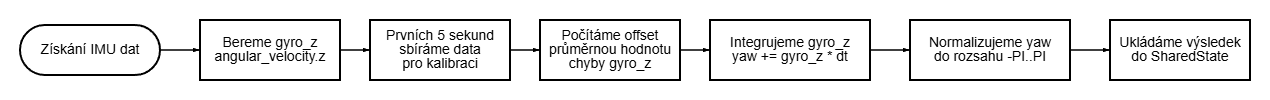
\includegraphics[width=0.9\linewidth]{figs/IMU_shema.png}
   \caption{Block schema IMU}
\end{figure}

\newpage

\subsection{Lidar}
Pro snímání vzdálenosti okolo robota je vužit lidar senzor, ze kterého selektujeme pět vzdáleností. Tři jsou použity na snímání stěn na regulaci robota a zjišťování překážky před sebou a dva jsou využity pro detekci křižovatek.

\begin{figure}[ht]
   \centering
   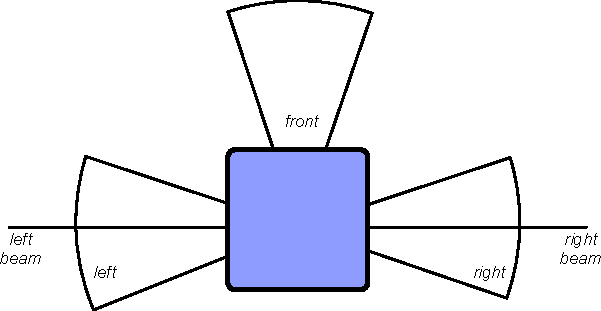
\includegraphics[width=0.5\linewidth]{figs/lidar.pdf}
   \caption{Úhly snímané lidarem}
\end{figure}

\begin{figure}[ht]
   \centering
   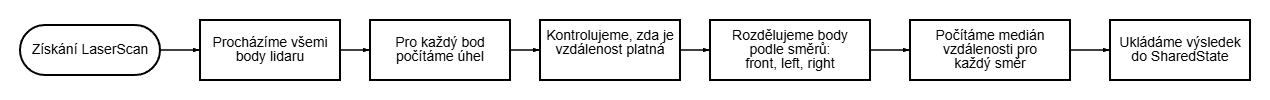
\includegraphics[width=0.8\linewidth]{figs/lidar.png}
   \caption{Block schema lidaru}
\end{figure}    

\section{Algoritmus}
Jako první při úniku z bludiště je nutné vykalibrovat IMU senzor, která probíhá automaticky po každém zapnutí programu. Po dokončení kalibrace je robot připravený vyjet a vyčkává na vstup od operátora a to zmáčknutím tlačítka na robotovi.
Po spuštění se řízení předá stavovému automatu.

\subsection{Kalibrace}
O správný chod programu se stará stavový automat, který je prvně ve stavu \verb|CALIBRATION|, jenž se stará o případ, pokud by bylo tlačítko na spuštění algoritmu zmáčknuto dříve, než byl IMU senzor zkalibrován.

Po úspěšné kalibraci se přejde do stavu \verb|CORRIDOR_NAVIGATION|. Zde se shromáždí data z lidaru a nastavují se příznaky, zda již byla viděna stěna na levé a pravé straně, toto slouží k zjištění, zda se nacházíme na křižovatce či nikoliv.

\subsection{PID}
Aby robot jezdil rovně a nenarážel do zdí se stará PID regulátor využívající lidaru a IMU. Lidar sleduje vzdálenost obou stran a pokud je v rozmezí, které odpovídá blízké stěně labyrintu tak se mezi sebou tyto hodnoty odečtou a podle velikosti rozdílu se robot kalibruje do středu. Při absenci z jedné stěn se využívá optimální vzdálenost od jedné snímané zdi, jen je síla této regulace snížena (\verb|wallError|). Regulaci ještě ovlivňuje IMU senzor, který se snaží o držení správného směru (\verb|headingError|).

\begin{equation*}
    correction = k_h * headingError + k_w + wallError    
\end{equation*}

\newpage

\subsection{Detekce křižovatek}
Za křižovatku považujeme jakoukoliv část bludiště, kde když se nacházíme, tak se můžeme vydat více směry (vlevo, vpravo a dopředu). Abychom zjistili zda se nacházíme na křižovatce se využívá příznak, který je v základu nastaven na \textit{false}. Při průjezdu v bludišti jsou kontrolovány, za pomocí dat z lidaru, vzdálenosti stran a překážky z předu robota. Pokud obě strany nebo alespoň jedna strana a vpředu volné, nacházíme se na křižovatce. Abychom předešli tomu, že se jedna křižovatka zdetekuje vícekrát, musí robot po zjištění, že je na křižovatce dostat data z lidaru, že minul někdy v pokračující jízdě stěny na obou dvou svých stranách.

\begin{figure}[ht]
   \centering
   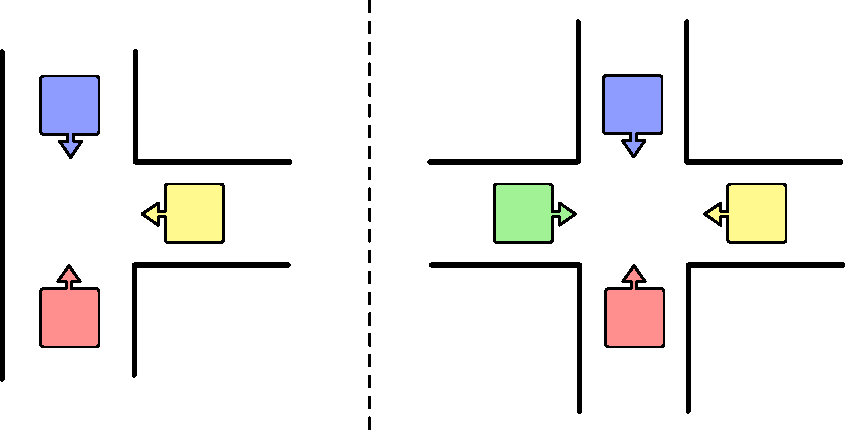
\includegraphics[width=0.7\linewidth]{figs/intersection.pdf}
   \caption{Dva typy křižovatek a možnosti odkud může robot přijet}
\end{figure}

\subsection{Aruco}
Když se robot nachází na křížení cest rozhoduje se kam pojede dál. K tomu slouží předem posbíraná data z kamery. Data jsou uložená v poli, kde se po nasnímání maximálně dvou kódu uloží a zde se využijí. Naše řešení má nastavenou prioritu na vyhledání pokladu a poté na útěk z bludiště. Pokud se žádný kód nenačte, nebo se načte špatně, robot se na křižovatce drží pravidla pravé ruky a to tedy pokud je možno odbočit vpravo, pokud nelze, pojede rovně. 

\subsection{Zatáčky}
Jestliže robot zaznamená překážku před sebou a nenachází se na křižovatce, je nutné zahnout. Směr zatáčení se určí podle toho, na jaké straně je nasnímána větší vzdálenost. O zatáčení se stará stav \verb|TURNING|, kde se využívá IMU senzor, který se otáčí o 90\degree oproti úhlu, který byl stanoven po poslední otočce robota. Po zatáčce je tedy nutno menší pauzy k ustálení robota a zapsání hodnoty z IMU.

\section{Závěr}
Robot s touto implementací byl schopen projet bludiště, získat poklad ubírající celkový čas a přitom nenabrat žádnou penalizaci.

\end{document}
